\section{Spatial Econometrics} 

\subsection{Background} 

\begin{frame}
	\frametitle{Immediate Plan}
 \begin{itemize}
 \item OLS estimation with diagnostics for spatial effects
 \item 2SLS estimation with diagnostics for spatial effects
 \item Spatial 2SLS for spatial lag model (with endogeneity)
 \item GM and GMM estimation for spatial error model
 \item GMM spatial error with heteroskedasticity
 \item Spatial HAC estimation
 \end{itemize}
 \end{frame} 

\begin{frame}
	\frametitle{Delivery}
 \begin{itemize}
 \item Freestanding
 \item Command line
 \item ArcGIS toolbox
 \end{itemize}
 \end{frame} 

\begin{frame}
	\frametitle{From pySpace to GeoDaSpace}
 
\begin{block}{First iteration}
 \begin{itemize}
 \item Had a fully functional version of GeoDaSpace
 \item Could not handle large problems $\rightarrow$ ~10,000 limit
 \item PySAL was not available $\rightarrow$ spatial weights
 \item Modularity $\rightarrow$ no reusable parts
 \end{itemize}
 \end{block} 
\begin{block}{Second iteration}
 \begin{itemize}
 \item Reuse the GUI nearly in its entirety
 \end{itemize}
 \end{block} \end{frame} 

\begin{frame}
	\frametitle{Loosely Coupled Framework}
  \begin{center}
  \includegraphics<1->[width=0.70\linewidth]{software_links.png}%
  \end{center}
 \end{frame} 

\subsection{PySAL} 

\begin{frame}
	\frametitle{PySAL Econometrics -- Setup OLS}
 \VerbatimInput[frame=single,numbers=left,numbersep=3pt,
 fontsize=\small]{figures/ols_commandLine.txt}
 \end{frame} 

\begin{frame}
	\frametitle{PySAL Econometrics -- Diagnostics Summary}
  \begin{center}
  \includegraphics<1->[width=0.53\linewidth]{ols_summary.png}%
  \end{center}
 \end{frame} 

\begin{frame}
	\frametitle{PySAL Econometrics -- Individual Diagnostics}
 \VerbatimInput[frame=single,numbers=left,numbersep=3pt,
 fontsize=\small]{figures/ols_diag.txt}
 \end{frame} 

\begin{frame}
	\frametitle{PySAL Econometrics -- Spatial Diagnostics}
 \VerbatimInput[frame=single,numbers=left,numbersep=3pt,
 fontsize=\small]{figures/spatial_diag.txt}
 \end{frame} 

\begin{frame}
	\frametitle{PySAL Econometrics -- Setup S2SLS}
 \VerbatimInput[frame=single,numbers=left,numbersep=3pt,
 fontsize=\small]{figures/s2sls_setup.txt}
 \end{frame} 

\subsection{GeoDaSpace} 

\begin{frame}
	\frametitle{Functionality}
 \begin{itemize}
 \item Spatial weights creation
 \item Spatially lagged variable computation
 \item GMM estimation methods
 \item Diagnostics
 \item Allow endogeneity
 \end{itemize}
 \end{frame} 

\begin{frame}
	\frametitle{User Interface}
  \begin{center}
  \includegraphics<1->[width=0.60\linewidth]{space1.png}%
  \llap{\includegraphics<2->[width=0.60\linewidth]{space2.png}}%
  \llap{\includegraphics<3->[width=0.50\linewidth]{spaceW.png}}%
  \llap{\includegraphics<4->[width=0.60\linewidth]{space3.png}}%
  \llap{\includegraphics<5->[width=0.20\linewidth]{spaceL.png}}%
  \llap{\includegraphics<6->[width=0.60\linewidth]{space4.png}}%
  \llap{\includegraphics<6->[width=0.20\linewidth]{spaceL.png}}%
  \llap{\includegraphics<7->[width=0.60\linewidth]{space5.png}}%
  \llap{\includegraphics<8->[width=0.80\linewidth]{spaceR.png}}%
  \llap{\includegraphics<9->[width=0.60\linewidth]{space4.png}}%
  \end{center}
 \end{frame} 

\begin{frame}
	\frametitle{(Near) Future}
 \begin{itemize}
 \item Spatial regimes
 \item Probit (classic and spatial)
 \item Maximum Likelihood
 \item Panel data
 \end{itemize}
 \end{frame} 


\section{Conclusion} 

\subsection{Next Steps} 

\begin{frame}
	\frametitle{PySAL Release Schedule}
 \begin{itemize}
 \item stuff
 \item stuff
 \item stuff
 \item stuff
 \end{itemize}
 \end{frame} 

\begin{frame}
	\frametitle{Other GeoDa Center Software}
 
\begin{block}{Currently Available}
 \begin{itemize}
 \item PySAL
 \item GeoDa (legacy)
 \item OpenGeoDa
 \item STARS
 \end{itemize}
 \end{block} 
\begin{block}{Coming Soon}
 \begin{itemize}
 \item GeoDaSpace
 \item GeoDaNet
 \item GeoDaWeight
 \item dynTM
 \end{itemize}
 \end{block} \end{frame} 

\begin{frame}
	\frametitle{Questions}
  \begin{center}
 \begin{figure}[htbp]
 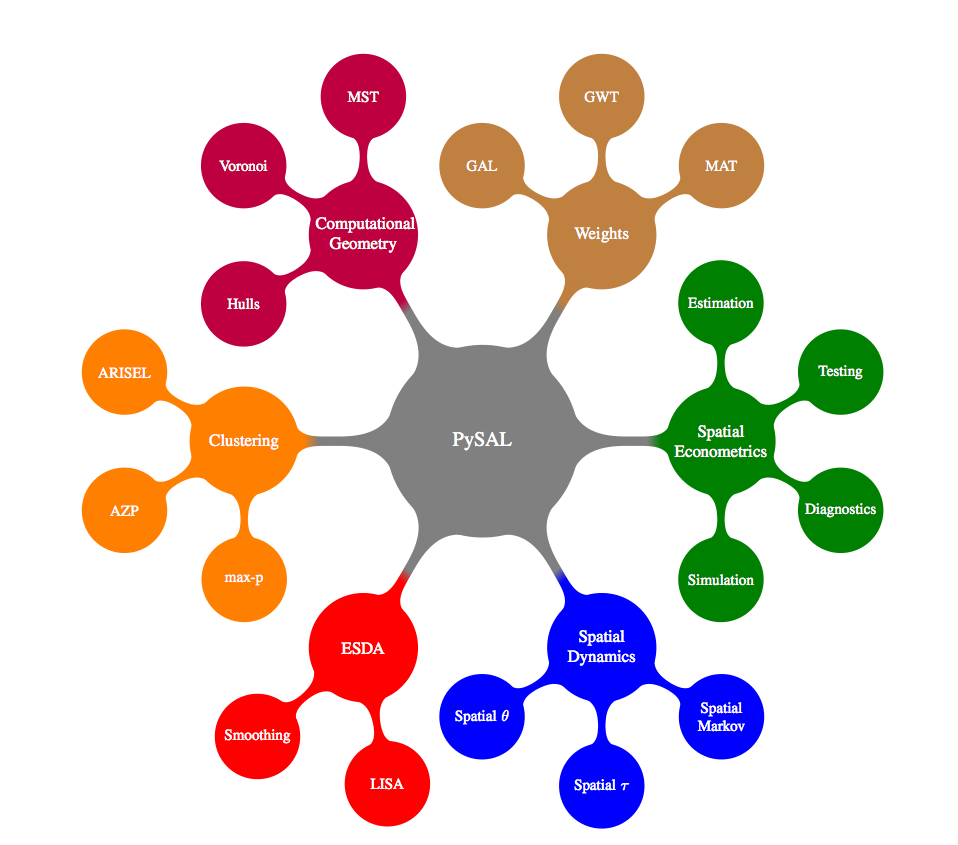
\includegraphics[width=0.60\linewidth]{pysalGraphic.png}
 \end{figure}
  {\color{blue}{\Large{geodacenter.asu.edu}}}\\
  {\color{blue}{\Large{www.pysal.org}}}
 \end{center}
 \end{frame} 



